\section{Background}

\begin{figure}[!htbp]
\centering
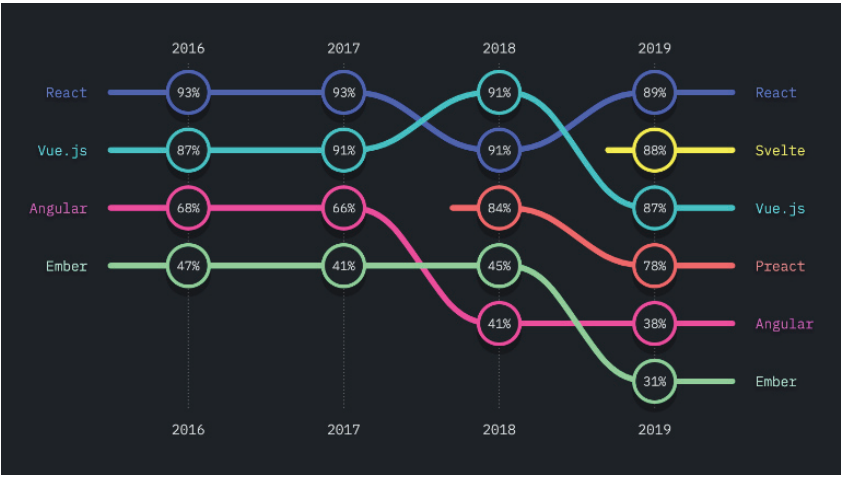
\includegraphics[width=\linewidth]{figs/popularity.png}
\caption{Popularity}
\label{fig:popularity}
\end{figure}

Representing the popularity trends of various web development frameworks over a period from 2016 to 2019

React, known for its robust ecosystem and backing by Facebook, has consistently held a significant share of popularity, while Vue.js has emerged as a strong contender with its approachable learning curve and incremental adoptability. Meanwhile, Svelte, the newest among them, presents an innovative approach by shifting work to compile time, leading to faster runtime performances.

To ensure a consistent standard of functionality across the web pages developed using each framework, Test-Driven Development (TDD) was employed as an aspect of our comparative analysis. This approach guaranteed that, although different frameworks were used, each implementation adhered to the same functional specifications. By integrating TDD into our workflow, we were able to provide a more objective measure of each framework's capabilities, taking into account not only the end product but also the development process itself.

In our analysis of front-end frameworks, we selected a weather application as our use case, primarily because it allows for practical experimentation with public APIs. This choice provided a tangible means to assess and compare the capabilities of various frameworks in handling real-time data, user interface dynamics, and responsiveness. The weather application scenario was particularly suited for this comparison as it involved fetching and displaying data from external sources, a common requirement in modern web development. This setup enabled us to evaluate how different the frameworks React, Svelte and Vue.js manage data binding, state management, and overall performance. Additionally, the integration with public APIs served as an excellent benchmark for understanding the ease of use, flexibility, and scalability offered by each framework, making our comparison comprehensive and relevant to current industry trends.

Central to our approach was the utilization of client-side operations, primarily fetching data from various APIs. The decision to not set up a dedicated backend allowed us to concentrate on the frontend functionalities, exploring how each framework handles tasks like API calls, data processing, and DOM manipulation. By simulating real-world scenarios where frontend applications interact with existing APIs, we were able to assess the efficiency, ease of integration, and responsiveness of each framework in handling client-side operations.

\subsection{Related Work}

Several studies and articles have compared the leading JavaScript frameworks, offering valuable insights for developers and researchers alike. The paper "Evaluating the Performance of Web Rendering Technologies Based on JavaScript: Angular, React, and Vue" presents a thorough comparative analysis focusing on performance metrics such as build size, time to interactive, and DOM manipulation time. It underscores Vue's superior performance in DOM manipulation and React's efficiency in interactivity, while noting Angular's larger bundle size. This study serves as a benchmark for understanding the technical strengths and limitations of these frameworks. (IEEE et al.)

An article on the DEV Community website further expands on this comparison by examining factors such as popularity, community support, and real-world applications of React, Vue, Angular, and Svelte​​ (Wichmann). It highlights the extensive communities and resources available for React and Angular, the moderate popularity of Vue, and the emerging presence of Svelte in the industry. The article also delves into performance assessments, aligning with the findings of the aforementioned study by highlighting the efficiency of Vue and Svelte​​​​.

Another critical aspect of these frameworks is the learning curve, as discussed in the Medium article by Faulkner Project, "Vue vs React vs Svelte" (Faulkner)​​. This article provides a practical perspective for new developers, emphasizing the user-friendly nature of Vue and Svelte compared to the more complex React. It also discusses real-world applications of these technologies, providing examples of companies that utilize them, thereby offering insights into their practicality in various industry settings​​​​​​.

Knowledge about different frontend frameworks is a critical asset for developers, preparing them to make discerning choices in a professional context and to deploy these tools adeptly in the creation of web solutions.

\subsection{Frameworks}

\subsubsection{About Vue:}

Vue.js is a modern, progressive JavaScript framework used for building user interfaces and single-page applications. It's known for its simplicity and gentle learning curve, which have contributed to a growing popularity among developers. Vue.js is approachable, performant, versatile, and designed to be incrementally adoptable. The core library is focused on the view layer only but can be easily integrated and scaled for complex applications using additional libraries and tooling​​ (Copes, 2018).

The framework facilitates the development process by offering a component-based architecture, allowing developers to create encapsulated and reusable components. Vue.js uses a declarative rendering model, where the developer writes templates in HTML that are bound to the underlying component state using a reactive and composable data binding system.

The design and implementation of Vue.js involve a balance of technical details and engineering trade-offs, which are well-documented and provide developers with a solid foundation for building applications. With Vue.js, components' data and DOM are reactively and efficiently updated, making state management straightforward and the development process more intuitive (HcySun, 2023, 1-574).


\subsubsection{About React:}

React, a JavaScript library developed by Facebook, has significantly transformed web application development. Its primary strength lies in its component-based architecture, which enables developers to build self-contained, state-managing components. This approach not only facilitates the creation of complex and reusable user interfaces but also as stated by (Novac et al. 1) that; “It is easy to build interactive applications with React.js because it makes views for each state of the application. When data is changed the framework React.js will perform the update and render the appropriate components.“

The library's declarative nature is another important part of its functionality. In React, developers define the desired state of the user interface, leaving the responsibility of actual DOM (Document Object Model) updates to React itself even though the paper Detecting code smells in React-based Webapps says that “React beginners usually use plain vanilla JavaScript to direct access a HTML DOM element, which can cause inconsistencies between React’s virtual DOM and the real DOM.” (Ferreira and Valente 5). This method ensures efficient rendering processes, as React compares the component's current state with its previous state and updates only the parts that have changed, not the entire page. Such an approach is particularly advantageous for the maintainability of large-scale applications, as it significantly enhances performance and streamlines the development workflow.

Moreover, React's lifecycle management provides developers with fine control over the behavior of components. This control is crucial for managing the various states in the application lifecycle, from initialization to updating and unmounting, allowing developers to execute specific code at each stage. The comprehensive ecosystem surrounding React, which includes tools like React Native for mobile app development and numerous third-party libraries, further extends its capabilities.

\subsubsection{About Svelte:}

Svelte, a groundbreaking framework in web development, was introduced by Rich Harris in 2016. It challenges traditional web development norms by shifting much of the work typically done in the browser to compile time. This results in highly optimized JavaScript code, setting Svelte apart from other frameworks like React and Vue. Svelte's approach is component-based, but it diverges notably in its operational philosophy, especially with its direct updates to the DOM instead of using a virtual DOM, leading to faster rendering and more efficient memory usage.

According to Bhardwaz and Godha, “Svelte also offers a more intuitive and straightforward way to build web applications. Instead of using a complex set of APIs, Svelte's syntax is easy to understand and follow, making it a great choice for developers who are new to web development.” (Bhardwaz and Godha, 2023, 1). Its syntax is cleaner and more intuitive, requiring less boilerplate code, which enhances code readability and maintainability. Svelte's reactive programming model is integrated into its language, streamlining state management and reducing reliance on external libraries.

Building upon the strengths of Svelte, SvelteKit (“Introduction • Docs • SvelteKit”) is a framework that I have been using, designed to create more complex and scalable web applications. SvelteKit extends Svelte's capabilities, providing server-side rendering, file-based routing, and full-stack capabilities. This makes SvelteKit a more complete solution for modern web development, allowing for the creation of both static sites and server-rendered applications with the same ease and efficiency that Svelte offers.
